\documentclass[a4paper, 12pt]{amsart}
\usepackage[french]{babel}
\usepackage[utf8]{inputenc}
\usepackage{amssymb}
\usepackage{graphicx}
\usepackage{coursebook}
\fthmstyle{plain}
\newfancythm{fthm}{Théorème}
\fthmstyle{defn}
\newfancythm{fdefn}{Définition}
\fthmstyle{ex}
\newfancythm{fex}{Exercice}
%\DeclareMathOperator*{\ln}{ln}
\newcommand{\pd}[2]{\ensuremath{\frac{\partial #1}{\partial #2}}}

\title{Eléments de correction pour les exercices vus en cours}

\begin{document}
\maketitle
\section{Mesure intégration}
\begin{fex}
Soit $(E,\mathcal{T},\mu)$ un espace mesuré avec $\mu(E)<+\infty$.
 Soit $f\colon E \to E$ une application mesurable. 
 On dit que $f$ préserve la mesure si $\forall A \in \mathcal{T},
\mu(f^{-1}(A))=\mu(A)$, et on supposera dans la suite
  que $f$ vérifie cette propriété.
Enfin, on notera, pour $n \geq 1$ et $A \subset E$: $f^{-n}(A)=\{x \in E \, | \,
f^n(x)\in A\}$  
avec $f^n=\underbrace{f \circ f \dots \circ f}_n$.
\begin{enumerate}
\item Montrer que pour tout $n \geq 1$, on a $\forall A \in  \mathcal{T},
\mu(f^{-n}(A))=\mu(A)$.
\item Pour $A \in \mathcal{T}$, on pose:
\[
H_A = \{ x \in A \, | \, \forall n \geq 1, f^n(x) \notin A \}
\]
Montrer que $H_A$ est mesurable.
\item Montrer que pour tout $n \geq 1$, on a $f^{-n}(H_A) \cap H_A = \emptyset$.
\item En déduire que pour tout couple d'entiers $(m,n), m \neq n$, on a:
\[
f^{-n}(H_A) \cap f^{-m}(H_A)= \emptyset
\]
\item Evaluer:
\[
\mu \left( \bigcup_{n \geq 0} f^{-n}(H_A) \right)
\]
et en déduire que $\mu(H_A)=0$. Ce résultat est connu sous le nom de théorème de
récurrence de Poincaré.
\end{enumerate}
\end{fex}
\begin{enumerate}
 \item Le plus simple est de raisonner par récurrence. La propriété est vraie
au rang $1$ par hypothèse. Supposons qu'elle soit vraie jusqu'au rang $n$. On a:
\[
 \mu\left(f^{-n+1}(A)\right) = \mu\left(f^{-1}\left(f^{-n}(A) \right) \right) =
\mu\left(f^{-n}(A)\right)
\]
en appliquant l'hypothèse de récurrence, $\mu\left(f^{-n}(A)\right)=\mu(A)$ ce
qui prouve le résultat demandé.
\item On remarque que:
\[
 H_A = A \cap \bigcap_{n \geq 1} f^{-n}\left({}^cA\right)
\]
On sait que ${}^cA$ est mesurable car $A$ l'est et donc 
$f^{-n}\left({}^cA\right)$ est mesurable par mesurabilité de l'application $f$.
Finalement, toute intersection dénombrable de parties mesurables étant
mesurable, on a $H_A$ mesurable.
\item Supposons l'existence de $x \in f^{-n}(H_A) \cap H_A$. Comme $x \in H_A$,
on a $f^{n}(x) \notin A$. Par ailleurs, $x \in f^{-n}(H_A)$, donc $f^{n}(x)\in
H_A \subset A$, qui est contradictoire.
\item On peut supposer que $n > m$, ce qui permet d'écrire:
\[
 f^{m}\left(f^{-n}(H_A) \cap f^{-m}(H_A)\right)= f^{-n+m}(H_A) \cap H_A =
\emptyset 
\]
La proposition s'en déduit.
\item La famille $f^{-n}\left(H_A\right), n\geq 0$ est formée d'ensembles
mesurables disjoints en vertu des questions précédentes. En application du
second axiome des mesures:
\[
 \mu \left( \bigcup_{n \geq 0} f^{-n}(H_A) \right) = \sum_{n \geq 0}
\mu\left(f^{-n}(H_A)\right) = \sum_{n \geq 0}
\mu\left(H_A\right)
\]
Comme la mesure de $E$ est finie, la série précédente doit l'être également, ce
qui implique $\mu\left(H_A\right) =0$.
\end{enumerate}
\begin{fex}
 On se place dans $\mathbb{N}$ que l'on munit de la tribu
$\mathcal{P}(\mathbb{N})$. 
\begin{enumerate}
  \item Montrer que l'application $\mu \colon A \in \mathcal{P}(\mathbb{N})
  \mapsto \#A$, avec $\#A$ le cardinal de $A$, est une mesure sur
  $\mathcal{P}(\mathbb{N})$.
  \item Montrer que les applications mesurables positives sur
  $\left(\mathbb{N},\mathcal{P}(\mathbb{N})\right)$ sont les suites de réels
  positifs.
  \item Soit $f=\left(f(0),f(1),\dots\right)$ une application mesurable positive
  sur $\left(\mathbb{N},\mathcal{P}(\mathbb{N})\right)$. Pour tout $n \in
  \mathbb{N}$, on pose:
  \[
  g_n = \left(f(0),f(1),\dots,f(n), 0, \dots \right)
  \]
  Montrer que pour tout $n \in \mathbb{N}$, $g_n$ est une application étagée
  positive et que la suite $(g_n)_{n \in \mathbb{N}}$ est croissante, de limite
  simple $f$.
  \item En déduire que:
  \[
  \int_{\mathbb{N}} f d \mu = \sum_{n=0}^{+\infty} f(n)
  \]
\end{enumerate}
\end{fex}
\begin{enumerate}
 \item On vérifie tout d'abord que $\mu(\emptyset)=\#\emptyset = 0$. Soit
$A_n,n\in \mathbb{N}$ une famille dénombrable de parties de $\N$ disjointes
deux à deux. Si l'une des parties est de cardinal infini, alors la réunion
l'est également et on a de façon triviale:
\[
\mu\left(\bigcup_{n \in \N}A_n\right) = \sum_{n \in \N} \mu(A_n) =+\infty
\]
Si maintenant toutes les parties sont de cardinal fini, soit il en existe un
nombre infini qui soient non vides, auquel cas le cardinal de la réunion est
infini, soit tous les $A_n$ sont vides au delà d'un certain rang, auquel cas on
a directement le fait que le cardinal de la réunion soit somme des cardinaux.
Dans ces deux cas on a encore:
\[
\mu\left(\bigcup_{n \in \N}A_n\right) = \sum_{n \in \N} \mu(A_n)
\]
prouvant que $\mu$ est une mesure.
\item Comme la tribu choisie est $\mathcal{P}(\N)$, toutes les applications de
$\N$ dans $\R$ sont mesurables. Une suite de réels étant précisément une telle
application, la propriéte demandée s'en déduit.
\item $g_n$ est une application mesurable ne prenant qu'un nombre fini de
valeurs distinctes, elle est donc étagée. La suite des applications $g_n$ est
bien évidemment croissante de limite simple $f$.
\item C'est la définition de l'intégrale d'une application mesurable positive à
partir des suites croissantes d'applications étagées (voir cours).
\end{enumerate}
\begin{fex}
 \begin{enumerate}
\item Soit la suite d'applications $(f_n)$ définies sur $[0,1]$ par~:
\[
\forall x \in [0,1], \, f_n(x) = \frac{nx}{1+n^2x^2}
\]
Déterminer la limite simple de cette suite. Conclure quant à la limite de~:
\[
\int_{[0,1]} f_n(x) d \lambda(x)
\]
\item On considère maintenant la suite $(g_n)$, applications définies sur
$\mathbb{R}$ par~:
\[
g_n(x) = \frac{1}{n} 1_{[0, n]}
\]
Déterminer la limite simple de cette suite. Peut-on appliquer le théorème de
convergence
dominée à~:
\[
\int_{\mathbb{R}} g_n(x) d\lambda(x)
\]
\end{enumerate}
\end{fex}
\begin{enumerate}
\item On a clairement $\forall x \in [0,1], \lim_n f_n(x) = 0$. Par ailleurs,
vérifiant que 
l'application~:
\[
u \to \frac{u}{1+u^2}
\]
atteint son maximum en $1$, on montre que~:
\[
\forall x \in [0,1], \, f_n(x) \leq \frac{1}{2}
\]
Comme l'application constante $\frac{1}{2}$ est sommable sur le compact $[0,1]$,
le théorème de
convergence dominée s'applique et~:
\[
\lim_n \int_{[0,1]} f_n(x) d \lambda(x) = 0
\]
\item Dans le deuxième cas, on a aussi convergence simple vers 0 (écrire la
définition!). Cependant, on n'a manifestement pas~:
\[
\lim_n \int_{\mathbb{R}} g_n(x) dx = 0
\]
chaque intégrale valant 1 !
Soit $g$ application telle que $\forall x \in \mathbb{R}, g(x) \geq
g_n(x)$. Il est clair que sur chaque intervalle $]n, n+1]$ on doit
avoir $g(x) \geq (n+1)^{-1}$. L'intégrale de $g$ sera donc minorée par
les sommes partielles de la série harmonique qui est divergente~: il
est impossible (heureusement !) d'appliquer la convergence dominée.
\end{enumerate}
\begin{fex}
Soit $f : \mathbb{R} \to \mathbb{R}$ une application sommable. On 
définit l'application $\phi : \mathbb{R} \to \mathbb{C}$ par~:
\[
\forall \xi \in \mathbb{R}, \, \phi(\xi) = \int_{\mathbb{R}} f(t) e^{-i 2 \pi
\xi t} d \lambda(t)
\]
\begin{enumerate}
\item Montrer que $\phi$ est bien définie et est continue sur $\mathbb{R}$.
\item On suppose maintenant que $f$ est telle que~:
\[
\int_{\mathbb{R}} | t f(t) | d \lambda(t) < +\infty
\]
Montrer que $\phi$ est dérivable et calculer sa dérivée.
\end{enumerate}
\end{fex}
\begin{enumerate}
\item L'existence de l'intégrale ne pose pas de problèmes~: $exp(-i 2 \pi \xi
t)$ est continue, donc mesurable. 
Le produit $f(t) exp(-i 2 \pi \xi t)$ est mesurable. Par ailleurs, $|f(t) exp(-i
2 \pi \xi t)| = |f(t)|$, d'où~:
\[
\int_{\mathbb{R}} |f(t) exp(-i 2 \pi \xi t)| d\lambda(t) = \int_{\mathbb{R}}
|f(t)| d \lambda(t) < +\infty
\]
par hypothèse.
La continuité découle de l'application immédiate du théorème de continuité des
intégrales dépendant d'un paramètre
vu en cours (reprendre les hypothèses).
\item Pour la dérivabilité, il convient d'écrire la forme la plus générale du
théorème de dérivation des intégrales dépendant d'un paramètre. Soit $\xi_0 \in
\mathbb{R}$~:
\begin{itemize}
\item L'application $F(t,\xi) = f(t) exp(-i 2 \pi \xi t)$ est sommable en $t$
pour tout $\xi$ réel.
\item Elle est dérivable en $\xi_0$.
\item On calcule~:
\begin{align*}
| f(t) e^{-i 2 \pi \xi t} - f(t) e^{- i 2 \pi \xi_0 t}| &= |f(t)||e^{-i 2 \pi
(\xi - \xi_0)t -1} \\
& \leq 2 \pi |t f(t)| |\xi - \xi_0|
\end{align*}
Comme $|t f(t)|$ est supposée sommable, les hypothèses du théorème sont
vérifiées ; la dérivée de 
l'intégrale en $\xi_0$ existe et vaut~:
\[
- i 2 \pi \int_{\mathbb{R}} t f(t) e^{-i 2 \pi x_0 t} d \lambda(t)
\]
\end{itemize}
\end{enumerate}
\begin{fex}
 On dit qu'une application $f : \mathbb{R} \to \mathbb{R}$ est
localement intégrable si elle est sommable sur tout compact de
$\mathbb{R}$. Soient $f,g$ localement intégrables. On pose~:
\[
F : x \to \int_0^x f(t) d \lambda(t) , \quad G : x \to \int_0^x g(t) d
\lambda(t)
\]
\begin{enumerate}
\item Montrer, en utilisant l'application~:
\[
h : (x,y) \to 1_{x \leq y} g(x) f(y)
\]
que pour tout intervalle borné $[a,b]$~:
\[
\int_{[a,b]} f(t)(G(t) - G(a)) d\lambda(t) =
\int_{[a,b]}g(t)(F(b)-F(t)) d\lambda(t)
\]
\item En déduire la formule d'intégration par parties~:
\[
\int_{[a,b]} F(t) g(t) d \lambda(t) = F(b)G(b)-F(a)G(a) - \int_{[a,b]}
f(t) G(t) d \lambda(t)
\]
\end{enumerate}
\end{fex}
La question 2) est une conséquence immédiate de la 1). On ne
détaillera que cette derniére.
$h$ est mesurable. En effet l'application:
\[
 (x,y) \in \R^2 \mapsto x \mapsto f(x)
\]
est mesurable comme composée de la projection canonique sur la première
composante et de $f$. De même pour l'application:
\[
 (x,y) \in \R^2 \mapsto y \mapsto g(y)
\]
Le produit de deux applications mesurables étant mesurable, on en déduit la
mesurabilité de $h$.
L'application $h$ est sommable sur $[a,b]^2$ car, par application du
théorème de Tonnelli~:
\begin{align*}
\int_{[a,b]^2} |h(x,y)| d \lambda \times d \lambda & \leq
\int_{[a,b]^2} |f(x)g(y)|  d \lambda \times d \lambda \\
& \leq \int_{[a,b]} |f| d \lambda \int_{[a,b]} |g| d \lambda < +\infty
\end{align*}
Le théorème de Fubini s'applique alors à $h$ et~:
\[
\int_{[a,b]} \left ( \int_{[a,b]} f(x,y) d \lambda(x) \right ) d
\lambda(y) = \int_{[a,b]} \left ( \int_{[a,b]} f(x,y) d \lambda(y)
\right ) d
\lambda(x)
\]
ce qui est précisément l'égalité demandée.

\begin{fex}
Soit $a>0, b>0$ deux réels strictement positifs. 
\begin{enumerate}
  \item Montrer que les deux intégrales
suivantes sont bien définies:
\[
\Gamma(a) = \int_{\mathbb{R}^+} e^{-x}x^{a-1} d\lambda(x) \, , \, B(a,b) =
\int_{[0,1]} x^{a-1}(1-x)^{b-1} d \lambda(x)
\]
\item Montrer que:
\[
\Gamma(a) = 2 \int_{\mathbb{R}^+} e^{-x^2} x^{2a-1} d \lambda(x)
\]
\item Justifier avec précision que:
\[
\Gamma(a)\Gamma(b) = 4 \int_{\mathbb{R}^{+2}}
e^{-(x^2+y^2)}x^{2a-1}y^{2b-1}d\lambda(x) d\lambda(y)
\]
\item En utilisant le changement de variable de l'exercice précédent, en
déduire:
\[
\Gamma(a)\Gamma(b)=B(a,b)\Gamma(a+b)
\]
\end{enumerate}
\end{fex}
\begin{enumerate}
 \item Les applications intégrées sont mesurables car continues et positives,
les intégrales existent donc. Elles sont toutes les deux finies: au voisinage
de 0 et 1 la sommabilité de $e^{-x}x^{a-1}$ (resp. $x^{a-1}(1-x)^{b-1}$)
s'obtient par application de l'échelle de comparaison de Riemann. La
sommabilité au voisinage de $+\infty$ de $e^{-x}x^{a-1}$ est un résultat
classique. En voici une preuve possible. On note tout d'abord que
$e^{-x}x^{a-1}=\exp\left((a-1)\ln x-x\right)$. Le logarithme étant concave sur
$\R^+$, son graphe est situé en dessous de toute tangente. Pour tout réel $x >
0$, on a donc:
\[
 \forall y \in \R^+, \, \ln y < \ln x + \frac{y-x}{x}
\]
Soit:
\[
\forall y \in \R^+, \, (a-1)\ln y -y < (a-1)(\ln x-1) +
y\left(\frac{a-1}{x}-1\right)
\]
Si $x=2(a-1)$, la majoration devient:
\[
 \forall y \in \R^+, \,  e^{-y}y^{a-1}< \exp\left((a-1)(\ln x-1)\right)
\exp\left(-\frac{y}{2}\right)
\]
qui est sommable au voisinage de $+\infty$.
\item Le changement de variable $x \mapsto x^2$ est un difféomorphisme de
classe $C^\infty$ sur $\R^{+*}$. En appliquant la formule du cours, on obtient
directement:
\[
 \Gamma(a) = 2 \int_{\mathbb{R}^+} e^{-x^2} x^{2a-1} d \lambda(x)
\]
\item L'application:
\[
 (x,y) \mapsto e^{-(x^2+y^2)}x^{2a-1}y^{2a-1}
\]
est continue sur $\R^{+*}\times \R^{+*}$, donc mesurable. Etant positive, on
peut appliquer Tonnelli:
\begin{align*}
  \int_{\mathbb{R}^{+2}}
& e^{-(x^2+y^2)}x^{2a-1}y^{2b-1}d\lambda(x) d\lambda(y) =  \\ &
\int_{\mathbb{R}^+} e^{-x^2} x^{2a-1} d \lambda(x) \int_{\mathbb{R}^+} e^{-y^2}
y^{2b-1} d \lambda(y)
\end{align*}
Ce qui prouve l'égalité demandée.
\item Le changement de variable en question utilise les coordonnées polaires
(exercice 16 du cours). C'est un difféomorphisme de classe $C^\infty$ de
$\R^{*+}\times ]0, \frac{\pi}{2}$ sur $\R^{+*}\times \R^{+*}$, d'expression:
\[
 \left(\rho,\theta\right) \mapsto \left(\rho \cos \theta, \rho \sin \theta 
\right)
\]
Le jacobien du changement de variable est $\rho$, ce qui donne, en application
de la formule du cours:
\begin{align*}
 & \int_{\mathbb{R}^{+2}}
e^{-(x^2+y^2)}x^{2a-1}y^{2b-1}d\lambda(x) d\lambda(y) = \\ &\int_{\R^{*+}\times
]0, \frac{\pi}{2}[} e^{-\rho^2}\rho^{2(a+b)-1} \cos^{2a-1}\theta
\sin^{2b-1}\theta d\rho d\theta
\end{align*}
En appliquant à nouveau Tonnelli, on peut intégrer par rapport à $\rho$ pour
faire apparaître $\gamma(a+b)$. Pour la seconde intégrale, on pose $t = \cos^2
\theta$, la formule du changement de variable donne:
\[
2\int_{]0, \frac{\pi}{2}[} \cos^{2a-1}\theta
\sin^{2b-1}\theta d\theta = \int_{]0,1[} t^{a-1}\left(1-t\right)^{b-1}dt =
B(a,b)
\]
Soit finalement:
\[
 \Gamma(a)\Gamma(b)=\Gamma(a+b)B(a,b)
\]
\begin{fex}
Déterminer les transformées de Fourier des applications suivantes~:
\[
\begin{array}{c}
f_1 \colon x \to e^{-|x|} \\
f_2 \colon x \to (1-|x|)1_{[-1,1]} \\
\end{array}
\]
\end{fex}
Les deux applications sont sommables, on utilise la formule du cours.
\begin{align*}
 \widehat{f_1}(\xi) & = \int_\R e^{-|x|-i\xi x } dx \\
& =  \int_{\R^+}e^{-x-i\xi x
} dx + \int_{\R^+}e^{x-i\xi x }
dx
\end{align*}
En utilisant une primitive pour les deux intégrales, il vient:
\[
  \widehat{f_1}(\xi) = \frac{1}{1+i\xi} + \frac{1}{1-i\xi} = \frac{2}{1+\xi^2}
\]
On vérifie la continuité et la décroissance à l'infini de l'application
obtenue. 
Pour $f_2$, on fait une intégration par parties:
\begin{align*}
 \widehat{f_2}(\xi) & = \int_{[0,1]} (1-x)e^{-i\xi x}dx +
\int_{[-1,0]}(1+x)e^{-i\xi x}dx \\
& = \left[ -\frac{(1-x)}{i\xi}e^{-i\xi x}\right]_0^1 + \left[
-\frac{(1+x)}{i\xi}e^{-i\xi x}\right]_{-1}^0 + \\
& \int_{[0,1]}\frac{-1}{i\xi} e^{-i\xi x} dx + \int_{[-1,0]}\frac{1}{i\xi}
e^{-i\xi x} dx
\end{align*}
Le terme intégré s'annule. Les deux intégrales restantes se calculent avec une
primitive. On obtient après simplification:
\[
 \widehat{f_2}(\xi) = \frac{2}{\xi^2}\left(1-\cos \xi \right)
\]
On vérifie continuité et décroissance en l'infini.
\end{enumerate}
\begin{fex}
\begin{enumerate}
  \item Déterminer la transformation de Fourier inverse dans $L^2(\mathbb{R})$
  de l'application $1_{[-1,1]}$.
  \item En déduire la transformation de Fourier de l'application $\sinc$:
  \[
  x \in \mathbb{R} \mapsto \sinc(x) = \left\{
  \begin{array}{cc}
  	1 & \text{ si } x=0 \\
  	\frac{\sin x}{x} & \text{ si } x \neq 0 
  \end{array}
  \right.
  \]
  \item Pouvez-vous en déduire que $\sinc \notin L^1(\mathbb{R})$ ?
\end{enumerate}
\end{fex}
\begin{enumerate}
 \item L'application proposée est sommable, on peut utiliser une intégrale pour
calculer sa transformée de Fourier inverse:
\[
 f \colon x \mapsto \frac{1}{2\pi}\int_{[-1,1]} e^{i \xi x } d \xi =
\frac{1}{\pi}\sinc x
\]
\item La transformée de Fourier étant inversible dans $L^2$, on en déduit
immédiatement que la transformée de Fourier de $\sinc$ est $\pi 1_{[-1,+1]}$.
\item La transformée trouvée n'est pas égale presque partout à une application
continue, elle ne peut donc
être obtenue à partir d'une application sommable.
\end{enumerate}
\begin{fex}
 Soit l'application~:
\[
f : x \to \left \{
\begin{array}{ll}
\frac{\sin^2 x }{x^2} & x \neq 0 \\
1 & x = 0
\end{array}
\right .
\]
\begin{enumerate}
\item Montrer que $f \in L^1(\mathbb{R})$ et calculer $\widehat{f}$
(on pourra utiliser la transformation inverse de Fourier dans
$L^2(\mathbb{R})$ de l'application $\pi 1_{[-1,+1]}$ vue dans l'exercice
précédent et le produit de convolution).
\item En déduire la valeur des l'intégrales~:
\[
\int_{\mathbb{R}} \frac{\sin^2 x}{x^2} d \lambda(x)
\]
et
\[
\int_{\mathbb{R}} \frac{\sin^4 x}{x^4} d \lambda(x)
\]
\end{enumerate}
\end{fex}
\begin{enumerate}
\item 
Comme $\sinc \in L^2(\mathbb{R})$, $f=\sinc^2  \in L^1(\mathbb{R})$. La
transformée de Fourier de $f$ s'obtient en utilisant la relation entre
produit de convolution et transformée de Fourier~:
\[
\widehat{f}*\widehat{g} = 2 \pi \widehat{fg}
\]
d'où~:
\[
\widehat{f} = \frac{\pi}{2} 1_{[-1,+1]} * 1_{[-1,+1]}
\]
soit~:
\[
\widehat{f}(\xi) = \frac{\pi}{2} 1_{[-2,+2]}(\xi)(2-|\xi|)
\]

\item La première intégrale est la valeur de $\widehat{f}$ en 0, soit
$\pi$. Pour la deuxième, on utilise la formule de Plancherel~: 
\[
2 \pi \|f\|_2^2 = \| \widehat{f} \|_2^2
\]
Le membre de droite se calcule aisément comme~:
\[
\frac{\pi^2}{2} \int_{[0,2]}(2-|\xi|)^2 d \lambda(\xi) = \frac{4 \pi^2}{3}
\]
soit~:
\[
\int_{\mathbb{R}} \frac{\sin^4 x}{x^4} d \lambda(x) = \frac{2 \pi}{3}
\]
\end{enumerate}
\section{Fonctions de la variable complexe}
\begin{fex}
 Soit $\Omega$ un domaine non vide de $\mathbb{C}$ et soit $f$ application
holomorphe sur $\Omega$. Montrer que les conditions suivantes sont
équivalentes~:
\renewcommand{\theenumi}{\alph{enumi}}
\begin{enumerate}
\item $f$ est constante sur $\Omega$.
\item $\Re(f)$ est constante sur $\Omega$.
\item $\Im(f)$ est constante sur $\Omega$.
\item $|f|$ est constante sur $\Omega$.
\end{enumerate}
\end{fex}
On séparera partie réelle et partie imaginaire de $f$ en posant $f=P+iQ$
Il est clair que (a) implique les autres conditions. Si on suppose (b), par
application des conditions de Cauchy et en utilisant que $P$ est constant:
\[
 \pd{P}{x} = \pd{Q}{y} = 0 , \pd{P}{y}=-\pd{Q}{x} = 0
\]
$\Omega$ étant connexe, on en déduit $Q$ constante. Il s'agit en fait d'une
équivalence $(b) \Leftrightarrow (c)$, le même raisonnement s'appliquant à $Q$.
On montre donc en sus que $|f|^2=P^2+Q^2$ est aussi une constante.
Finalement, si l'on suppose $P^2+Q^2$ constant, les dérivées partielles de
cette application par rapport à $x,y$ donnent;
\[
 P\pd{P}{x}+Q\pd{Q}{x}= 0,\,  P\pd{P}{y}+Q\pd{Q}{y}= 0
\]
En utilisant les conditions de Cauchy:
\[
 P\pd{P}{x}-Q\pd{P}{y}= 0,\,  P\pd{P}{y}+Q\pd{P}{x}= 0
\]
Il s'agit d'un système linéaire homogène de déterminant $P^2+Q^2=|f|^2$. Si
cette quantité est nulle, alors $f$ est nulle et (a) est vérifiée. Sinon:
\[
 \pd{P}{x}=\pd{P}{y}=0
\]
prouvant que $P$ est une constante et donc aussi $Q$ car $(b) \Leftrightarrow
(c)$, soit $f$ constante.
\begin{fex}
 Soit la série entière:
\[
f \colon z \mapsto \sum_{n >0}(-1)^{n-1}\frac{(z-1)^n}{n}
\]
\begin{enumerate}
  \item Déterminer son rayon de convergence;
  \item Montrer que pour tout réel $x \in ]0,2[$, $f(x)=\log(x)$;
  \item En déduire que $f$ est l'unique application analytique prolongeant le
  logarithme réel sur le disque ouvert $B(1,1)$;
  \item Vérifier que sur $B(1,1)$, on a $\exp \circ f = Id$.
\end{enumerate}
\end{fex}
\begin{enumerate}
 \item On utilise le critère de d'Alembert. Le rapport de deux termes
consécutifs est $n/(n+1)$, de limite 1 à l'infini. Le rayon de convergence est
donc 1.
\item Résultat classique de classes préparatoires. On peut dériver terme à
terme la série dans son disque ouvert de convergence, qui donne la série:
\[
\sum_{n >0}(-1)^{n} (z-1)^n = \frac{1}{1+(z-1)}
\]
La valeur particulière $f(1)=0$ permet alors de conclure.
\item $f$ coïncide avec $\log$ sur une partie possèdant un point d'accumulation
(en fait, tout le segment réel $]0,2[$). Par le principe du prolongement
analytique, elle est unique.
\item Toujours sur le segment $]0,2[$, $\exp \circ f = \exp \circ \log = Id$.
Par prolongement analytique de l'application $\exp \circ f$, cette égalité est
vraie sur $B(1,1)$.
\end{enumerate}
\begin{fex}
 Soit l'application $f \colon z \mapsto \exp\left(i z^2\right)$. 
\begin{enumerate}
  \item Montrer que $f$ est holomorphe sur $\mathbb{C}$ et vérifier que sa
  dérivée est continue.
  \item Pour tout réel $r > 0$, le contour $\gamma_r$ est défini selon la figure
  \ref{fig:contour2}. Proposer une écriture de $\gamma_r$ sous la forme d'une
  courbe de Jordan régulière de classe $C^1$ par morceaux.
  \item Que vaut l'intégrale:
  \[
  \int_{\gamma_r} f(z) dz
  \]
  \item Ecrire cette intégrale sous la forme d'une somme de trois
  intégrales de chemin et montrer que l'intégrale correspondant à l'arc de
  cercle tend vers 0 lorsque $r \to +\infty$.
  \item En déduire les valeurs des intégrales généralisées suivantes, dites
  intégrales de Fresnel:
  \[
  \lim_{r \to +\infty} \int_{[-r,r]} \cos(x^2) dx, \quad  \lim_{r \to +\infty}
  \int_{[-r,r]} \sin(x^2) dx
  \]
\end{enumerate}
\end{fex}
 \begin{figure}[ht]
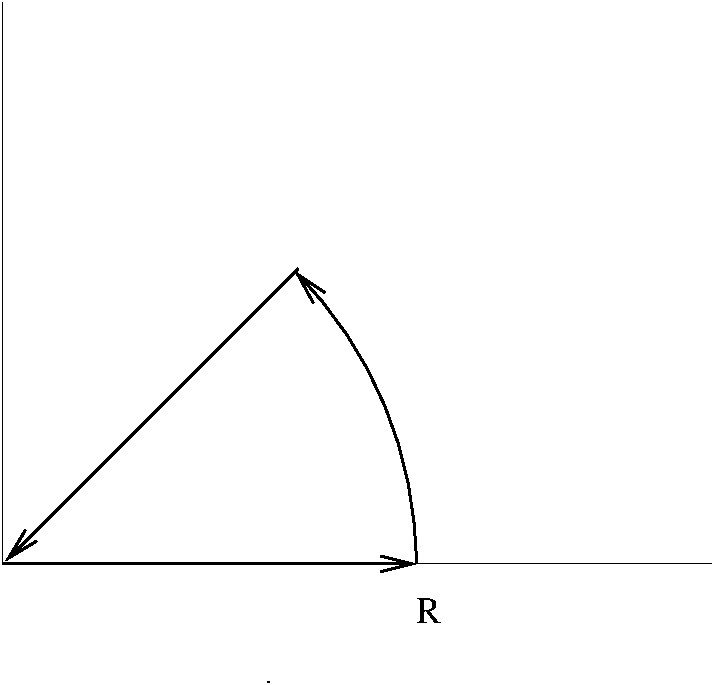
\includegraphics[scale=0.3]{contour_fresnel.pdf}
\caption{Contour $\gamma_r$}\label{fig:contour2}
\end{figure}
\begin{enumerate}
\item L'application $f$ est holomorphe comme composée d'applications
holomorphes. Sa dérivée est $f^\prime(z) = 2 i z f(z)$, qui est continue. 
\item
Par la formule de Cauchy, on a~:
\[
\int_{\gamma_3 . \gamma_2 . \gamma_1} f(z) dz = 0
\]
Par ailleurs~:
\[
\int_{[0,R]} e^{ix^2}d \lambda(x) = \int_{\gamma_1} f(z) dz
\]
En choisissant pour $\gamma_2$ le paramètrage~:
\[
t \in [0, \frac{\pi}{4}] \to \gamma_2(t) = e^{it}
\]
on obtient~:
\[
\int_{\gamma_2} f(z) dz = \int_{[0, \frac{\pi}{4}]} e^{-R^2 \sin (2t)
+ i R^2 \cos(2t)} i R e^{it} d \lambda(t)
\]
On peut majorer le module de $\int_{\gamma_2} f(z) dz$ par~:
\[
\int_{[0, \frac{\pi}{4}]} e^{-R^2 \sin (2t)}  R d \lambda(t)
\]
Comme l'application $\sin$ est concave sur $[0, \frac{\pi}{2}]$, sur
cet intervalle on a~: $\sin(t) \geq \frac{2 t}{\pi}$, ce qui donne la
majoration~:
\[
\left | \int_{\gamma_2} f(z) dz \right | \leq 
\int_{[0, \frac{\pi}{4}]} e^{-\frac{R^2 4 t}{\pi}} R dt =
\frac{(\pi)(1- e^{-R^2})}{4 R}
\]
\item
\[
\int_{\gamma_3} f(z) dz = e^{i \frac{\pi}{4}} \int_{[0,R]} e^{-t^2} d\lambda(t)
\]
d'où en passant à la limite et en remarquant que $\lim_{R \to
+\infty}\int_{\gamma_2} f(z) dz = 0$~:
\[
I = J = \frac{1}{2} \sqrt{\frac{\pi}{2}}
\]
\end{enumerate}
\begin{fex}
 Soit $f \colon z \in \mathbb{C} \mapsto \exp(-z^2)$.
\begin{enumerate}
  \item Montrer que $f$ est holomorphe dans $\mathbb{C}$, de dérivée continue.
  \item En utilisant le contour $\gamma_r$ donné figure \ref{fig:contour3},
déterminer, pour
  $\omega \in \mathbb{R}$ fixé, la valeur de l'intégrale:
  \[
  \int_{\gamma_r} \exp(-z^2)dz
  \]
  \item En faisant tendre $r$ vers $+\infty$ et en faisant un raisonnement
  similaire à celui de l'exercice précédent, déterminer la transformée de
  Fourier de l'application $x \mapsto \exp(-x^2)$.
\end{enumerate}
\end{fex}
 \begin{figure}[ht]
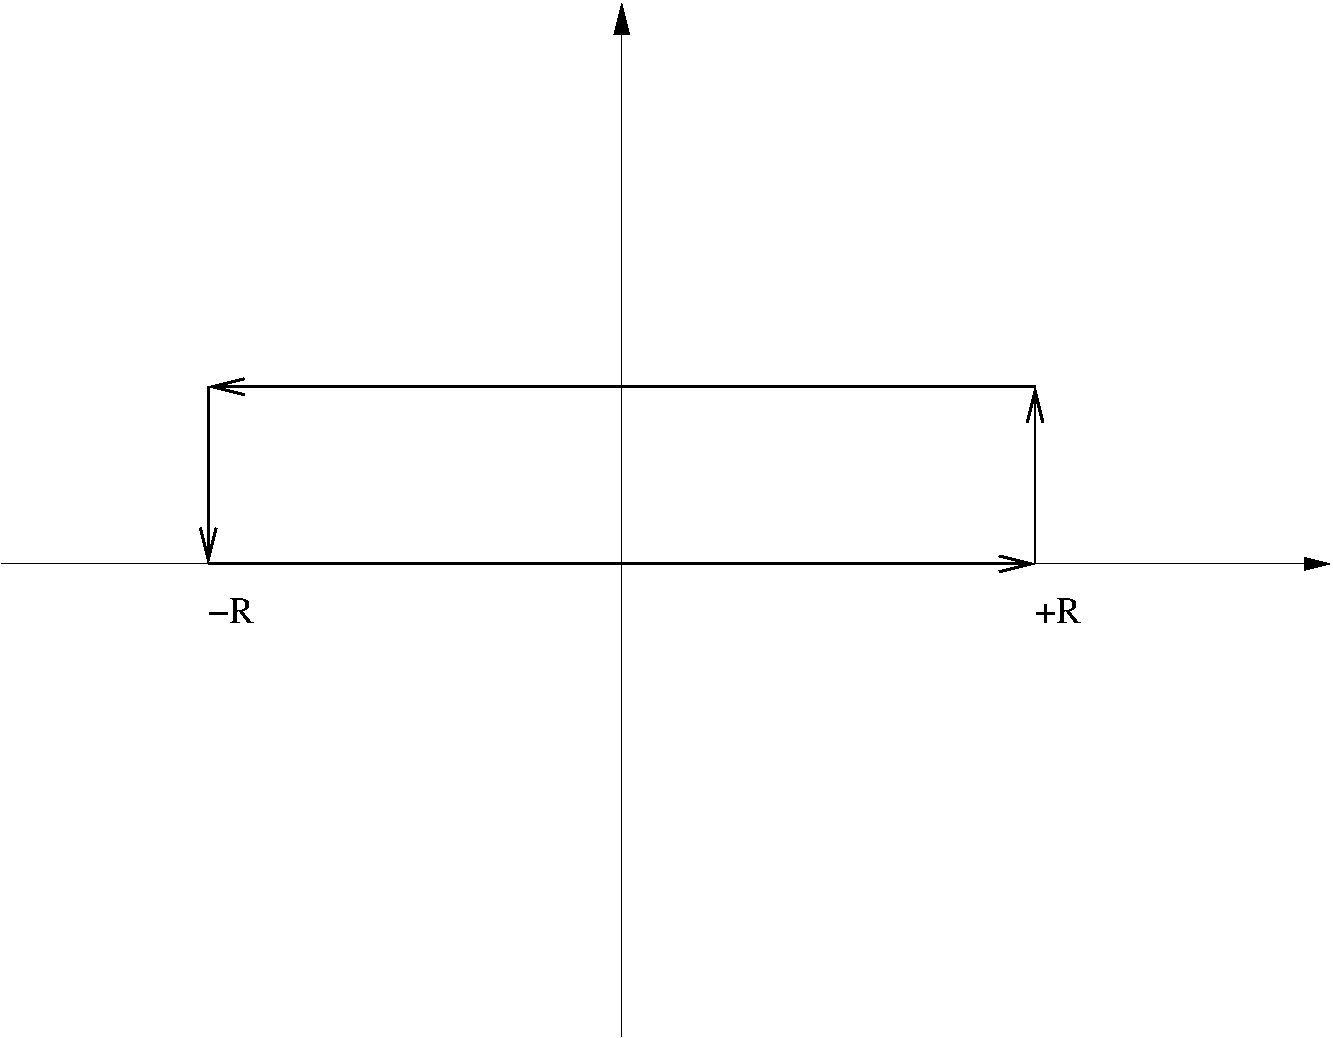
\includegraphics[scale=0.3]{contour_gauss.pdf}
\caption{Contour $\gamma_r$}\label{fig:contour3}
\end{figure}
\begin{enumerate}
 \item Même raisonnement que dans l'exercice précédent.
\item L'application intégrée est holomorphe, la formule de Cauchy s'applique:
\[
  \int_{\gamma_r} \exp(-z^2)dz = 0
  \]
\item L'intégrale sur l'axe réel est:
\[
 \int_{[-r,r]} \exp(-x^2) dx 
\]
de limite $\sqrt{\pi}$ pour $r \to +\infty$. Le segment supérieur se paramètre
par:
\[
 t \in [-r,r] \mapsto -t+i \frac{\omega}{2}
\]
L'intégrale le long de ce chemin est donc:
\[
 - \int_{[-r,r]} e^{-t^2 + i t \omega + \frac{\omega^2}{4}} dt
\]
La limite lorsque $r\to +\infty$ est:
\[
- e^{\frac{\omega^2}{4}} \int_\R  e^{-t^2 + i t \omega} dt 
\]

Finalement, l'intégrale sur les segments verticaux aura pour limite $0$ si $r
\to +\infty$. Un paramétrage possible du segment situé en $r$ est:
\[
t \in [0, \frac{\omega}{2}] \mapsto r + it 
\]
conduisant à l'intégrale:
\[
 i \int_{[0, \frac{\omega}{2}]} e^{-(r+it)^2} dt 
\]
son module se majore par:
\[
 \frac{\omega}{2}e^{-r^2 + \frac{\omega^2}{4}}
\]
qui a bien pour limite $0$ lorsque $r \to +\infty$. Le second segment vertical
se traite de la même façon. En regroupant les termes et en remarquant que la
transformée de Fourier est une application paire, on en déduit finalement
qu'il s'agit de l'application:
\[
 \xi \mapsto \sqrt{\pi} e^{-\frac{\omega^2}{4}}
\]
\end{enumerate}
\begin{fex}
Soit $f$ l'application définie par:
\[
f \colon z \mapsto \frac{\exp(iaz)}{1+z^2}
\]
avec $a>0$ réel. 
\begin{enumerate}
  \item En utilisant la première formule de Cauchy, évaluer l'intégrale de $f$
  le long du contour donné figure \ref{fig:contour_ex1} et sous l'hypothèse
  $R>1$.
  \item Par passage à la limite $R \to +\infty$, en déduire la transformée de
  Fourier de l'application $x \mapsto (1+x^2)^{-1}$.
\end{enumerate}
\end{fex}
\begin{figure}[ht]
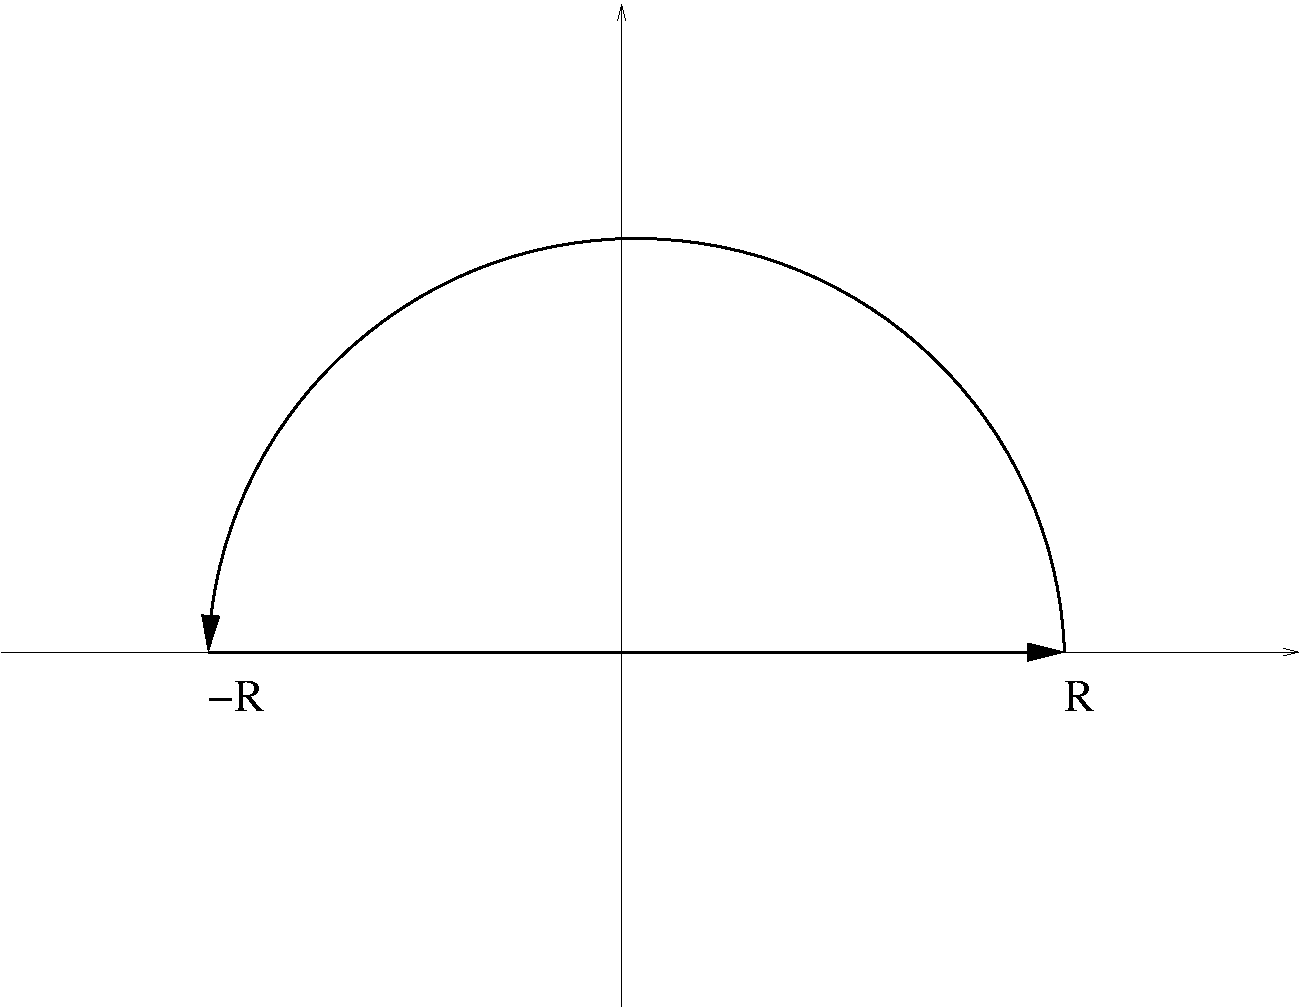
\includegraphics[scale=0.3]{contour_ex1.pdf}
\caption{Contour d'intégration}\label{fig:contour_ex1}
\end{figure}
\begin{enumerate}
 \item Pour $R > 1$, le point $i$ se trouve à l'intérieur du contour
d'intégration $\gamma$. On a donc:
\[
 \int_\gamma \frac{\exp(iaz)}{z+i} \frac{dz}{z-i} = i 2 \pi \frac{\exp(-a)}{2i}
= \pi \exp(-a)
\]
\item On applique le lemme de Jordan:
\[
\left|z\frac{\exp(iaz)}{z^2+1}\right| = \frac{|z|\exp(-a\Im(z))}{|1+z^2|}
\]
Sur le demi-cercle, $\Im(z) \leq 0$, d'où:
\[
\frac{|z|\exp(-a\Im(z))}{|1+z^2|} \leq \frac{R}{R^2-1}
\]
qui a pour limite 0 lorsque $R \to +\infty$.
\item On obtient immédiatement que pour $\xi > 0$, la transformée de Fourier a
pour valeur $\pi \exp(-\xi)$. Par parité, elle vaut donc sur tout $\R$,
$\pi \exp(-|\xi|)$.

\end{enumerate}
\begin{fex}
 Calculer les intégrales généralisées suivantes~:
\[
\begin{array}{l}
I_1 = \int_0^{+\infty} \frac{x^2 \cos(ax)}{1+x^4} dx , \quad a \in
\mathbb{R}\\
I_2 = \int_0^{+\infty} \frac{ \sin x}{x}dx
\end{array}
\]
\end{fex}
L'intégrale $I_1$ est absolument convergente~:
\[
\left |  \frac{x^2 \cos(ax)}{1+x^4} \right | \leq \frac{x^2}{1+x^4}
\]
On supposera $a\geq0$ en toute généralité puisque le cosinus est une application
paire.
Soit $f_1 : z \to \frac{z^2 e^{iaz}}{1+z^4}$ que l'on intégre sur le contour
de l'exercice précédent.
Le lemme de Jordan s'applique directement sur le demi-cercle~:
\[
\left |
\frac{z^3 e^{iaz}}{1+z^4} 
\right | \leq \frac{|z|^3 e^{-a \Im(z)}}{|1-|z|^4|}
\]
Les pôles de $f$ dans le domaine intérieur au contour sont, pour $R$ assez
grand~:
\[
z_1 = e^{i\frac{\pi}{4}}, \, z_2 = e^{i\frac{3\pi}{4}}
\]
On utilise la formule du cours pour calculer le résidu d'une fraction
rationnelle en un pôle simple~: 
\[
Res(z_k) = \frac{z_k^2 e^{ia z_k}}{4 z_k^3}
\]
On en déduit après calculs~:
\[
I_1 = \frac{4 \pi e^{-a/\sqrt{2}}}{\sqrt{2}} \left (
\sin\frac{a}{\sqrt{2}} - \cos \frac{a}{\sqrt{2}} \right )
\]
Pour la seconde intégrale,
On utilise l'application $g : z \to \frac{e^{iz}}{z}$ et le contour donné en
figure \ref{fig:contour_sinc}. 
Elle est
holomorphe dans le domaine intérieur au contour. Par continuité
de $g$, la  limite de l'intégrale
sur le demi-cercle intérieur lorsque le rayon tend vers 0 est $\pi$. 
Sur le
demi-cercle extérieur (de rayon $R$), on majore l'intégrale par~:
\[
2 \int_{[0, \frac{\pi}{2}]} e^{- \frac{2 R t}{\pi}} d\lambda(t)
\]
qui tend vers 0 pour $R \to + \infty$. On en déduit que la valeur de
l'intégrale généralisée demandée est $\frac{\pi}{2}$.
\begin{figure}[ht]
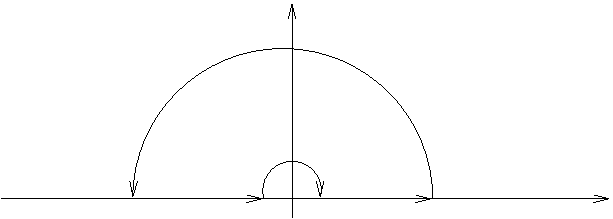
\includegraphics[scale=1]{contour_sinc.pdf}
\caption{Contour d'intégration}\label{fig:contour_sinc}
\end{figure}
\end{document}